\documentclass[article]{jss}
\usepackage{comment}
\usepackage{graphicx}
\usepackage{tikz}
\usetikzlibrary{shadows,trees}
\usepackage{fancyvrb}
\usepackage{cprotect}

\usepackage[firstpage]{draftwatermark}
\SetWatermarkLightness{.95}
%%%%%%%%%%%%%%%%%%%%%%%%%%%%%%
%% declarations for jss.cls %%%%%%%%%%%%%%%%%%%%%%%%%%%%%%%%%%%%%%%%%%
%%%%%%%%%%%%%%%%%%%%%%%%%%%%%%

%XXX To add
% simpleVisitor to see the sequence of cursor kinds
% Clean up the macros in the protect.tex example.  (Done?)


%% almost as usual
\author{Duncan Temple Lang\\University of California at Davis}
\title{RCIndex: Querying C/\protect\Cpp Code in R with libclang}

%% for pretty printing and a nice hypersummary also set:
\Plainauthor{Duncan Temple Lang}
\Plaintitle{RCIndex: Querying C/C++ Code in R with libclang}
\Shorttitle{RCIndex}

%% an abstract and keywords
\Abstract{ 

The ability to get information about \C/\Cpp{} code routines and data
structures can allow us to do many things in an intrepreted language
such as \R.  We use \libclang{}, a flexible, embeddable library, to
develop \R{} functionality to obtain and use information about native
code.  We describe the \Rpkg{RCIndex} package which provides
high-level functionality to access and utilize this information and
also lower-level approaches to query and manipulate other aspects of
native source code.  We describe how to use the package and scenarios in
which it is useful.  This functionality is infrastructural and some of
the functionality of the package is the native code analogy to the
\Rpkg{codetools} package for \R{} code.  It is not necessarily of
direct interest to end-users, but it allows us to build numerous tools
that can help end-users and developers.

} 
\Keywords{\R, \Rpkg{RCIndex} package, compiled code, meta-data,
  bindings}  %, software metrics}
\Plainkeywords{R, RCIndex package, compiled code, meta-data, bindings} %% without formatting
%% at least one keyword must be supplied

%% publication information
%% NOTE: Typically, this can be left commented and will be filled out by the technical editor
%% \Volume{13}
%% \Issue{9}
%% \Month{September}
%% \Year{2004}
%% \Submitdate{2004-09-29}
%% \Acceptdate{2004-09-29}

%% The address of (at least) one author should be given
%% in the following format:
\Address{
  Duncan Temple Lang\\
  4210 Math Sciences Building, \\
  University of California at Davis \\
  One Shields Avenue\\
  Davis, CA 95616\\
  E-mail: \email{duncan@r-project.org}\\
  URL: \url{http://www.omegahat.org}
}

\usepackage{xspace}
\usepackage{relsize}

\usepackage[T1]{fontenc} 
\catcode`\_=12

\def\llvm{LLVM}
\def\C{C}
\def\perl{\proglang{PERL}}
%\def\Cpp{\proglang{C$++$}}
% See http://tex.stackexchange.com/questions/4302/prettiest-way-to-typeset-c-cplusplus
%\newcommand{\Cpp}{C\nolinebreak\hspace{-.05em}\raisebox{.4ex}{\tiny\bf +}\nolinebreak\hspace{-.10em}\raisebox{.4ex}{\tiny\bf +}\xspace}
\newcommand\Cpp{C\nolinebreak[4]\hspace{-.05em}\raisebox{.4ex}{\relsize{-3}{\textbf{++}}}\xspace}
%\def\Cpp{{C\nolinebreak[4]\hspace{-.05em}\raisebox{.4ex}{\tiny\bf ++}}}
\def\Java{\proglang{Java}}
\def\Python{\proglang{Python}}
\def\R{\proglang{R}}
\def\S{\proglang{S}}
\def\Splus{\proglang{S-PLUS}}
\def\llvm{\proglang{LLVM}}
\def\Rpkg#1{\pkg{#1}}
\def\Rfunc#1{\textsl{#1()}}
\def\Rop#1{\texttt{#1}}
\def\Rdollar{\texttt{\$}}
\def\Rvar#1{\textsl{#1}}
\def\Rel#1{\textbf{#1}}
\def\Cfunc#1{\textit{#1()}}
\def\Cvar#1{\textit{#1}}
\def\file#1{\textbf{#1}}
\def\dir#1{\textbf{#1}/}
\def\Ctype#1{\texttt{#1}}
\def\Rclass#1{\textit{#1}}
\def\Rslot#1{\textbf{#1}}
\def\Rarg#1{\textbf{#1}}
\def\Roption#1{\dquote{\textsl{#1}}}
\def\Rkeyword#1{\textbf{\textsl{#1}}}
\def\Cppkeyword#1{\textbf{#1}}
\def\Ckeyword#1{\textbf{#1}}
\def\Carg#1{\textbf{\textsl{#1}}}
\def\Cexpr#1{\textsl{#1}}
\def\Rexpr#1{\textit{#1}}

\def\Rtrue{TRUE}
\def\Rfalse{FALSE}

\def\libclang{\textbf{libclang}}
\def\clang{\textbf{clang}}
\def\gcc{\textit{GCC}}
\def\XML{\textit{XML}}

\def\dquote#1{``#1''}

\def\ShFlag#1{\textit{#1}}

\def\libclangFlag#1{-\nolinebreak\texttt{#1}}

\def\ClangKind#1{\textit{#1}}
\def\ClangTypeKind#1{\textsl{#1}}

\DefineVerbatimEnvironment{RCode}{Verbatim}{fontshape=sl}
\DefineVerbatimEnvironment{CCode}{Verbatim}{fontshape=tt}
\DefineVerbatimEnvironment{ShCode}{Verbatim}{fontshape=it}
\DefineVerbatimEnvironment{ROutput}{Verbatim}{fontshape=bf}

\begin{document}

%XXX connect with codetools

\section{Motivation}\label{sec:Introduction}

We typically think of \C{} and \Cpp code as something we write,
compile and call. It is rarely the input to anything but the compiler.
However, such code is a source of potentially useful information that
we can exploit in statistical and scientific computing.  
%XXX Give  some vague hints as to what these are.
In order to
leverage this information, we need to be able to access it in a
structured manner and in a form that we can compute on and in the
programming environment in which we want to use it.
\libclang{}~\citep{bib:libclang,bib:libclangSlides} has
emerged as a powerful, industrial-strength library that provides
valuable functionality for working with \C/\Cpp source code and which
we can embed in \R{} (and many other languages).

There are several applications of being able to programmatically
understand \C/\Cpp code in a high-level language such as \R.

\textbf{Registering \R-callable routines}: When we write \C/\Cpp
code to use in an \R{} package, it is useful to explicitly register
the routines that we can call via any of the
\Rfunc{.C}/\Rfunc{.Call}/\Rfunc{.External} interfaces.  When the
routines are registered, \R{} can help to identify potential errors in
calling them.  \R{} can detect an incorrect number of arguments for a
routine, or that the types are incorrect, e.g., an integer vector when
a numeric vector is expected. Registration also allows us to resolve
the symbols just once rather than each time we call a routine, and it
also allows us to use different symbols/names to refer to the routines.  It
is convenient to be able to run \R{} code to identify the \R-callable
routines and to generate the registration information
programmatically.  As we change these routines, we can programatically
update the registration information with little effort and ensure the
information is synchronized.


\textbf{Generating bindings to native libraries}: Numerous \R{}
packages provide interfaces to existing \C/\Cpp libraries.  This
typically involves manually creating two pieces of code. The first is
an \R-callable wrapper routine corresponding to each routine of
interest in the third-party library. The second is a corresponding
\R{} function that invokes the wrapper routine, having coerced the
\R{} arguments to the appropriate form.  This is often quite
straightforward, but both time-consuming and error-prone.  This makes
for unnecessarily lengthy write-debug-test cycles.  Instead, we'd like
to be able to programmatically read the information about the
third-party routines and data types and then generate all of the code.
We want to minimize human intervention.  If we could generate these
``bindings'' programmatically, the \R{} programmer can spend time
creating higher-level functionality using these primitives.

\textbf{Dynamic calls to native routines}: The
\Rpkg{rdyncall}~\citep{bib:rdyncall} and \Rpkg{Rffi}~\citep{bib:Rffi}
\R{} packages avoid having to explicitly create the wrapper routines
and \R{} functions to interface to existing \C{} routines. Instead,
they both provide a dynamic mechanism to call arbitrary native
routines.  However, both approaches require a description of the
target routines.  Again, we want to obtain this information
programmatically and then we can easily generate these descriptions
and remove humans from the process.

\textbf{Understanding third-party libraries interactively}: When we
interface to third-party libraries, we typically read documentation to
identify and understand the important routines and data structures.
In some situations, it can be convenient to find this information
interactively within an environment such as \R.  Rather than reading
static document, we can query the code for information such as how
often a particular data type is returned by a routine or passed as an
argument? or what idioms does the library use?  We can use \R's
graphics capabilities to visualize the code and which routines call
which other routines.

%documentation in comments - see RCUDA.
\textbf{In-line documentation as comments}: Often third-party native
libraries contain documentation in comments adjacent to the corresponding
routines and data structures.  Accordingly, it is convenient to be able to easily
access this documentation and potentially reuse it as \R{}
documentation for functions that interface to the routines, as we did
for the \Rpkg{RCUDA} package (\url{http://github.com/duncantl/RCUDA}).

\textbf{Compiling \R{} code}: Recently, we have been developing \R{}
facilities for compiling \R{} code to native instructions to by-pass
the \R{} interpreter.  This allows us to rewrite and translate \R{}
code so that it is essentially native code and can call other existing
native routines, for example, in the \R{} engine or standard \C{}
libraries.  This results in significant speedup.  However, to make
this work, we need to know the signature -- parameter types and return
type -- of these native, external routines.  Again, if we can find
this information programmatically, we greatly simplify and improve the
entire process of generating the code.


%XXX Tighten this up. First sentence is not quite connected to second.
\textbf{Determining memory management and mutability of inputs and
  outputs}: When we call existing native routines, we often need
to know whether we are in charge of the memory for the inputs or
whether the called routine is responsible.  Often, programmers omit
important information about whether a parameter is modified within a
routine or if it is constant.  This is important information as it
allows us to differentiate between an array of values passed as a
pointer, or a scalar whose contents are changed.  We would like to be
able to analyze the body of the routine to be able to determine if and
how it modifies its parameters so that we can avoid making copies of
data, if possible.


\textbf{Software as Data}: While we may not think of code as data,
analyzing software is an important field of research and industry.
Software defines several networks related to i) which routines call
which other routines, ii) the hierarchical structure of \Cpp
classes, iii) which files \texttt{\#include} other files, and so on.
We can explore how these networks change over time, i.e., modifications
to the code. We can find which global/non-local variables are used in
which routines to help identify problems with parallelization and
potential refactorzation of the code.  We can combine this data with
version control history to better understand software projects.


\textbf{Detecting errors in native code for \R}: \R's package
mechanism provides a powerful set of tests and checks for potential
errors in \R{} code.  These are very useful and can identify errors
such as misspelled variable or function names before the code is run.
It would be valuable to perform analogous tests on \C{} code in \R{}
packages.  We might identify common issues such as not protecting
allocated \R{} objects from garbage collection.  We could do this by
analyzing uses of \Cfunc{PROTECT} and \Cfunc{UNPROTECT} calls and
ensuring there is an appropriate correspondence.  These are
\R-specific checks and will not be done by other code-analyzing
software, e.g., the compiler.


We can also find ``dead'' routines that are never called by other
routines and so help to reduce the code.

We hope these applications motivate the utility of being able to
navigate native code in \R{} and indicate that there are many more.  In
this paper, we describe how to use the \R{} interface to \libclang{} to
find this kind of information needed in these types applications.  We
start next by describing the fundamental concepts of \libclang{} in
section~\ref{sec:libclangConcepts}.  We follow this in
section~\ref{sec:RCIndex} by introducing the high-level functionality
provided by the \Rpkg{RCIndex} package, e.g., getting the routines,
data structures, \Cpp classes in a source file.  We then discuss the
lower-level functionality in the package on which these higher-level
functions are based in section~\ref{sec:BuildingBlocks}. 
%XXX say why for the previous sentence, i.e., so people can adapt and
%extend the high functionality.
 We explore
three reasonably comprehensive examples or case-studies in
section~\ref{sec:Examples} and then compare this approach with others
that I and others have pursued in the past.  Finally, we outline some
future plans for the package and its use.




% This could come after the high-level material, but it may make sense here.
\section[Concepts of libclang]{Concepts of \libclang}\label{sec:libclangConcepts}

%Translation units,  AST and cursors, traversing the tree, types
Before we discuss the \R{} facilities for working with \libclang, it
is useful to understand the basic concepts of the library.  These
include translation units, abstract syntax trees and cursors, types
and tokens.  \libclang{} exposes other concepts, but those are not  the
important ones for our purposes.

Source code is arranged in files. A project may be made up of more
than one related files. %XXX grammar
For example, we may define related routines
for one task in one file and other routines in a separate file.
Header files are used for declarations and pre-processor definitions
that are shared by several files.  When we parse a file, the parser
essentially reads the source and substitutes the content of any header
files referenced by an \Ckeyword{\#include} directive directly into
the source.  The entity resulting from parsing the document is called
a \textit{translation unit} (TU).


\libclang{} is a parser and represents a translation unit as a parse
tree where the nodes are called \textit{cursors}.  It first breaks the
text into tokens during the lexical analysis step.  This breaks code
of the form \Cexpr{dnorm(n, 1, sd)} into the separate tokens
\dquote{dnorm}, \dquote{(}, \dquote{n}, \dquote{1}, \dquote{sd},
\dquote{)}.  The parsing stage then maps the tokens into language
concepts represented by different kinds of cursors.  In this example,
the concept is a call expression. Within the call entity is the
reference to the routine being called -- \Cfunc{dnorm} -- and then the
three arguments to the call.  The parenthesis and comma tokens
disappear in the parsing stage as we move from the individual tokens
to higher-level semantic meaning of the tokens.  However, a cursor
still has access to its original tokens and we can obtain these for a
given cursor. This turns out to be important as \libclang{} doesn't
differentiate between different types of binary operators, for
example. Instead, we find the operation (=, +, -, etc.)  from the
tokens and so the concepts of both cursor and token are important.
%XXX the last few sentences could be written better.  Too specific
% so make the point more gracefully.

\libclang{} represents the different parse elements 
%XXX elements of the parsed content
via a cursor (of
class \Rclass{CXCursor} in \R).  A cursor has a kind that identifies
its nature or what concept it represents. There are many different
kinds for a cursor (enumerated in the variable \Rvar{CXCursorKind} in
the \Rpkg{RCIndex} package) and they include FunctionDecl, VarDecl,
ParmDecl, CallExpr, IntegerLiteral, ClassDecl, MacroDefinition,
EnumDecl, StructDecl.  Hopefully the names indicate the purpose of the
cursor.

\begin{figure}
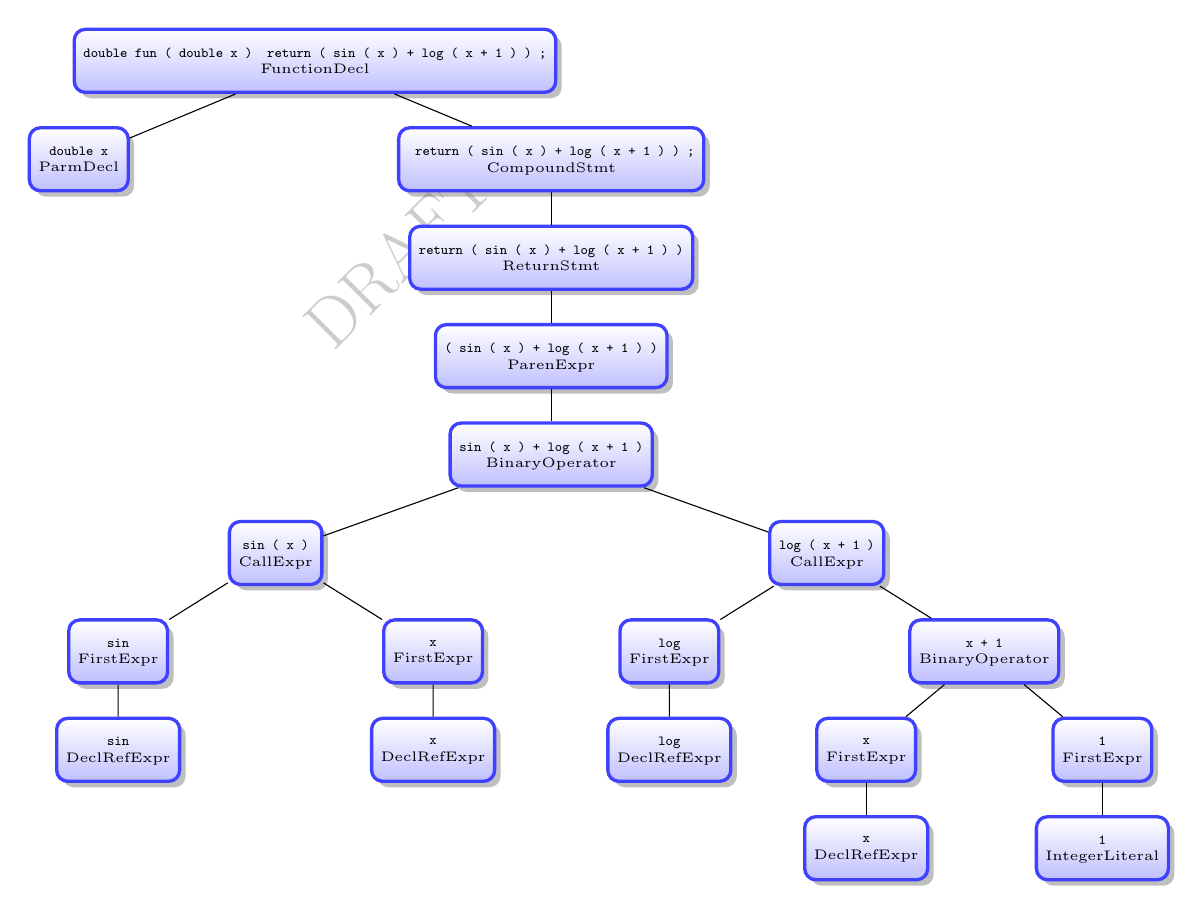
\begin{tikzpicture}
[
font=\tiny,
level distance=1.25cm,
level distance=1.25cm,
every node/.style={top color=white,
    bottom color=blue!25,
    rectangle,rounded corners,
    minimum height=8mm,
    draw=blue!75,
    very thick,
    drop shadow,
    align=center,
    text depth = 0pt},
 level/.style={sibling distance=6cm},
 level 4/.style={sibling distance=7cm},
 level 5/.style={sibling distance=7cm},
 level 6/.style={sibling distance=4cm},
 level 7/.style={sibling distance=3cm}
]
 \node {\Verb!double fun ( double x )  return ( sin ( x ) + log ( x + 1 ) ) ;!\\ FunctionDecl}
 child {
  node {\Verb!double x!\\ ParmDecl}
 }
 child {
  node {\Verb! return ( sin ( x ) + log ( x + 1 ) ) ;!\\ CompoundStmt}
  child {
   node {\Verb!return ( sin ( x ) + log ( x + 1 ) )!\\ ReturnStmt}
   child {
    node {\Verb!( sin ( x ) + log ( x + 1 ) )!\\ ParenExpr}
    child {
     node {\Verb!sin ( x ) + log ( x + 1 )!\\ BinaryOperator}
     child {
      node {\Verb!sin ( x )!\\ CallExpr}
      child {
       node {\Verb!sin!\\ FirstExpr}
       child {
        node {\Verb!sin!\\ DeclRefExpr}
       }
      }
      child {
       node {\Verb!x!\\ FirstExpr}
       child {
        node {\Verb!x!\\ DeclRefExpr}
       }
      }
     }
     child {
      node {\Verb!log ( x + 1 )!\\ CallExpr}
      child {
       node {\Verb!log!\\ FirstExpr}
       child {
        node {\Verb!log!\\ DeclRefExpr}
       }
      }
      child {
       node {\Verb!x + 1!\\ BinaryOperator}
       child {
        node {\Verb!x!\\ FirstExpr}
        child {
         node {\Verb!x!\\ DeclRefExpr}
        }
       }
       child {
        node {\Verb!1!\\ FirstExpr}
        child {
         node {\Verb!1!\\ IntegerLiteral}
        }
       }
      }
     }
    }
   }
  }
 }
;
\end{tikzpicture}
  
\cprotect\caption{This shows the structure of a cursor tree for the 
\C{} routine \Cfunc{sinLog} shown in figure~\ref{fig:sinLogRoutine}.
Each node in the tree shows the kind of the cursor
and the text of the expression with which it is associated.
The cursor kind \dquote{FirstExpr} essentially means unexposed or hidden.
}
\label{fig:sinLogTree}  
\end{figure}

\begin{figure}
\centering
\begin{CCode}
              double
              sinLog(double x)
              {
                 return(sin(x) + log(x + 1));
              }
\end{CCode}  

\caption{A simple routine that takes a single \Ctype{double} value
and returns a new value. Figure~\ref{fig:sinLogTree} illustrates the
parse tree for this routine.}\label{fig:sinLogRoutine}
\end{figure}


Along with its kind, a cursor has child cursors.  These are the
components such as the reference to the routine and the parameters in
a call, the fields and methods in a \Cpp{} class or the left and right
hand side of an assignment expression. Each of these child cursors has
a kind and also, possibly, its own sub-cursors. As a result, we have a
tree, or hierarchical structure.  Figure~\ref{fig:sinLogTree}
illustrates this hierachy for a simple routine shown in
figure~\ref{fig:sinLogRoutine}, along with the kind of cursor and 
its expression.  The translation unit is the
container for the top-most or root cursor of the tree.  This root
cursor has the abstract kind \ClangKind{TranslationUnit}.  Its
children are the top-level elements of the source code file,
e.g. global variables, routines, class definitions, pre-processor
terms. Each of these has its own child cursors and so on.

This concept of a cursor tree is important when we examine how to
extract information using the lower-level facilities in
sections~\ref{sec:BuildingBlocks}~and~\ref{sec:Examples}.  We will traverse
the tree, either one node at a time or directly by querying child
cursors and their children.

In addition to cursors, \libclang{} manages type information.  In the
\C{} and \Cpp{} languages, every expression has a type, be it a
variable declaration, a call to a routine, a binary operator, and so on.  \libclang{}
associates a type with each cursor.  Importantly, it ensures that
there is a single type object describing each unique data type in the
translation unit, and across related translation units.  This allows
us to reason about and resolve types quite easily.

Like a cursor, a \libclang{} type has a kind such as \ClangTypeKind{Int},
\ClangTypeKind{Float}, \ClangTypeKind{Double},
\ClangTypeKind{Typedef}, \ClangTypeKind{Pointer},
\ClangTypeKind{Record} (for a \Ckeyword{struct}),
\ClangTypeKind{Enum}.  A type also has a name, a size (number of
bytes) and other characteristics we can query.


A translation unit contains all the information from the corresponding
source file.  A single TU is often sufficient for our purpose of
exploration and analysis. However, if the code in one translation unit
refers to routines or variables in an other source file, we have to
merge it with another translation unit to resolve those references.
\libclang{} uses an \textit{index} as the container for several
related translation units.  When we want to deal with the translation
units together, we use the same index to parse them and this then
allows \libclang{} and us to connect references to elements across
translation units.


\libclang{} provides other features such as diagnostics for both parsing
and compiler errors, code completion used in editors, serializing
translation units, precompiled header files and efficient indexing of
one or more translation units.  Some of these are exposed in the \Rpkg{RCIndex}
package. However, none are essential for understanding how to work
with \libclang{} and extracting useful information from source code.






\section[The RCIndex package]{The \Rpkg{RCIndex} package}\label{sec:RCIndex}
The \Rpkg{RCIndex} provides numerous high-level functions that return
information about \C{} code.  These refer to functions that I have
developed building on the lower-level tools and which users can call
to get useful information directly or to perform high-level tasks such
as generating registration information or getting all the routines or
\Cpp classes in a source file. These might be initial steps in a
higher-level task, but these are high-level relative to the primitive
functions in the \Rpkg{RCIndex} package with which we implemented
these functions.
%XXX iron out these sentences.

\subsection{High-level Functionality}

% Talk about filtering based on the file name. (Implement this
% consistently).  Mention can do it afterwords or during the collection.

We might consider functions that take a source file and extract one or
more of the types of top-level elements in that file, e.g., routines,
data structures, enumeration definitions, \Cpp class definitions as
the very highest-level functions.  The \R{} user can call these
functions with just the name of the file and perhaps additional
arguments for the parser and the results are returned.  The user
doesn't have to write any code to manipulate or traverse the parse
tree (AST).  She doesn't have to necessarily create a translation unit
before calling one of these functions. As such, they are ``atomic''.
These functions can also take an existing, previously parsed,
translation unit rather than the file name.  This is useful if we are
going to make multiple separate queries of the same source code,
i.e., we parse it once and query it multiple time.

The following paragraphs describe many of the high-level functions in
the \Rpkg{RCIndex} package.

\paragraph{Finding routines}
The \Rfunc{getRoutines} does as its name suggests. It takes a file
name or an existing translation unit object and returns a list with an
element for each routine declaration or definition in the
corresponding code.  Each element contains the \Rclass{CXCursor}
object representing the routine, a list of the parameters giving their
name and data types, and the return type.  This is an S4
object of class \Rclass{FunctionDecl}. Since this contains the cursor,
we can query it for the name of the routine, the file in which it is
located, the location in that file and so on. In other words,
information that we don't explicitly collect into the \R{} object can
be determined later when we use this description of the routine.
%?Show example?

\paragraph{Data type definitions}
The routines are typically our focus so that we can invoke them from
\R{} or analyze their code. However, the routines work on data types
and therefore we need to be able to find the definitions of these data
types.  The \Rfunc{getDataStructures} function returns a list of the
data types defined in a translation unit corresponding to a source
file.  These include \Ckeyword{struct} and \Ckeyword{union}
definitions, \Ckeyword{typedef}s for providing an alternative name for
an existing type and enumerated constant definitions.

\paragraph{\protect\Cpp class definitions}
For \Cpp code, we can use \Rfunc{getCppClasses} to traverse a
translation unit, either pre-parsed or a source file, and construct a
description for each of the \Cpp classes it contains. Each class
description is an instance of the class \Rclass{C++Class} in \R, with
template classes using the derived class \Rclass{TemplateC++Class}.  A
class description contains the name of the class, a list of its fields
and another for its methods, and references to the base/super class
cursors.  The fields and methods each have their type information and
also the accessor qualifier, i.e., \Cppkeyword{private},
\Cppkeyword{protected} or \Cppkeyword{public}.  It is relatively
straightforward to generate \Cpp code from this description that
defines a new derived sub-class whose methods we can implement with \R{}
functions.  We can then provide \R{} instances of that class that
operate transparently as regular \Cpp objects.


\paragraph{Enumerated constant definitions}
\Rfunc{getEnums} returns a list of the enumeration definitions in a
source file, i.e., corresponding to an expression of the form
\Cexpr{enum \{ A, B, C\}}. Each element is an instance of the S4 class
\Rclass{EnumerationDefinition}.  Like the \Rclass{FunctionDecl} class,
this contains a reference to the definition in case we want to query
it further at a later time.  The actual values in the enumeration are
stored in the \Rslot{values} slot as a named integer vector.  The
names are the symbolic names we should use, while the values are the
literal values to which these names correspond.  These values allow us
to cross the interface between \R{} and native code where there is no
existing association between the symbolic names and the literal values.

\paragraph{Global Variables}
The \Rfunc{getGlobalVariables} function returns information about all
of the top-level/non-local variables within a source file.  From this, we have
their names and types, and can also determine if they are constant,
and if they are local to this file (i.e., \Ckeyword{static}) or
accessible to routines in other files.  We may be interested in global
variables for various reasons.  We can use either of the
\Rpkg{rdyncall} or \Rpkg{Rffi} packages to dynamically access the
current value of a global variable.  We also want to remove global
variables when making code thread-safe or just for improving the logic
of the code, i.e., avoiding side-effects.

The function \Rfunc{findGlobals} finds global variables that are used
within a routine or entire translation unit.  The function is
intentionally analogous to the \Rfunc{findGlobals} function in
\Rpkg{codetools}~\citep{bib:codetools}. It returns the variables, and
optionally, the routines that are called, within a routine/translation
unit which are not locally defined as parameters or local variables.


\paragraph{Find calls to routines}
The \Rfunc{findCalls} function takes a cursor -- typically either a
routine or an entire translation unit -- and finds the names of
routines in any call made within this code.  This allows us to
determine which routines call which other routines and so describe a
graph/network.  We can then discover potentially interesting things
about the routines.  For example, we might look at just the routines
within a single file and see which of these call other routines in the
file and which are called by other routines in the file.  This might
identify isolated routines that don't necessarily belong in this
particular file. It might also help us to understand how the the
routines interact and cluster.  We can use the \Rpkg{igraph}~\citep{bib:igraph} and/or
\Rpkg{graph}~\citep{bib:graphPkg} packages to perform computations on the network and also
to visualize it.

%XXX so this is the first place we have an example.
% Should we have examples earlier on, i.e., for the previous examples.
We'll show how to do this on a file \file{memory.c} in the \R{}
interpreter's source.
We start by obtaining the routines from the file:
\begin{RCode}
f = sprintf("%s/../src/main/memory.c", R.home())
r = getRoutines(f, args = "-DHAVE_CONFIG_H",
                  includes = c(sprintf("%s/../src/include", R.home()),
                               sprintf("%s/include", R.home())))
\end{RCode}
We'll discuss the extra arguments \Rarg{args} and \Rarg{includes} in section~\ref{sec:BuildingBlocks}.

For each of these routines, we find which routines they call with
\begin{RCode}
kalls = lapply(r, findCalls)
\end{RCode}
To restrict the routines to only those within this file
and create the adjacency matrix, we use 
\begin{RCode}
withinFileCalls = lapply(kalls, intersect, names(r))    
m = matrix(0, length(r), length(r), dimnames = list(names(r), names(r)))
invisible(sapply(names(withinFileCalls), 
           function(id) 
              m[id,  withinFileCalls[[id]]] <<- 1))
\end{RCode}
We'll discard the routines that are not called by any other routine
and themselves do not call any routine in the file. We do this with
\begin{RCode}
i = rowSums(m) == 0 & colSums(m) == 0
m = m[!i, !i]  
\end{RCode}
These are all basic \R{} manipulations of \R{} objects and have
nothing to do with \libclang.

% We could do this more elegantly.
Finally, we can draw the graph
\begin{RCode}
library(igraph)
g = graph.adjacency(m, "directed")       
plot(g, vertex.size = 2, vertex.label.cex = .6, edge.arrow.size = .5)
\end{RCode}
and it is displayed in figure~\ref{fig:callgraph}.

\begin{figure}
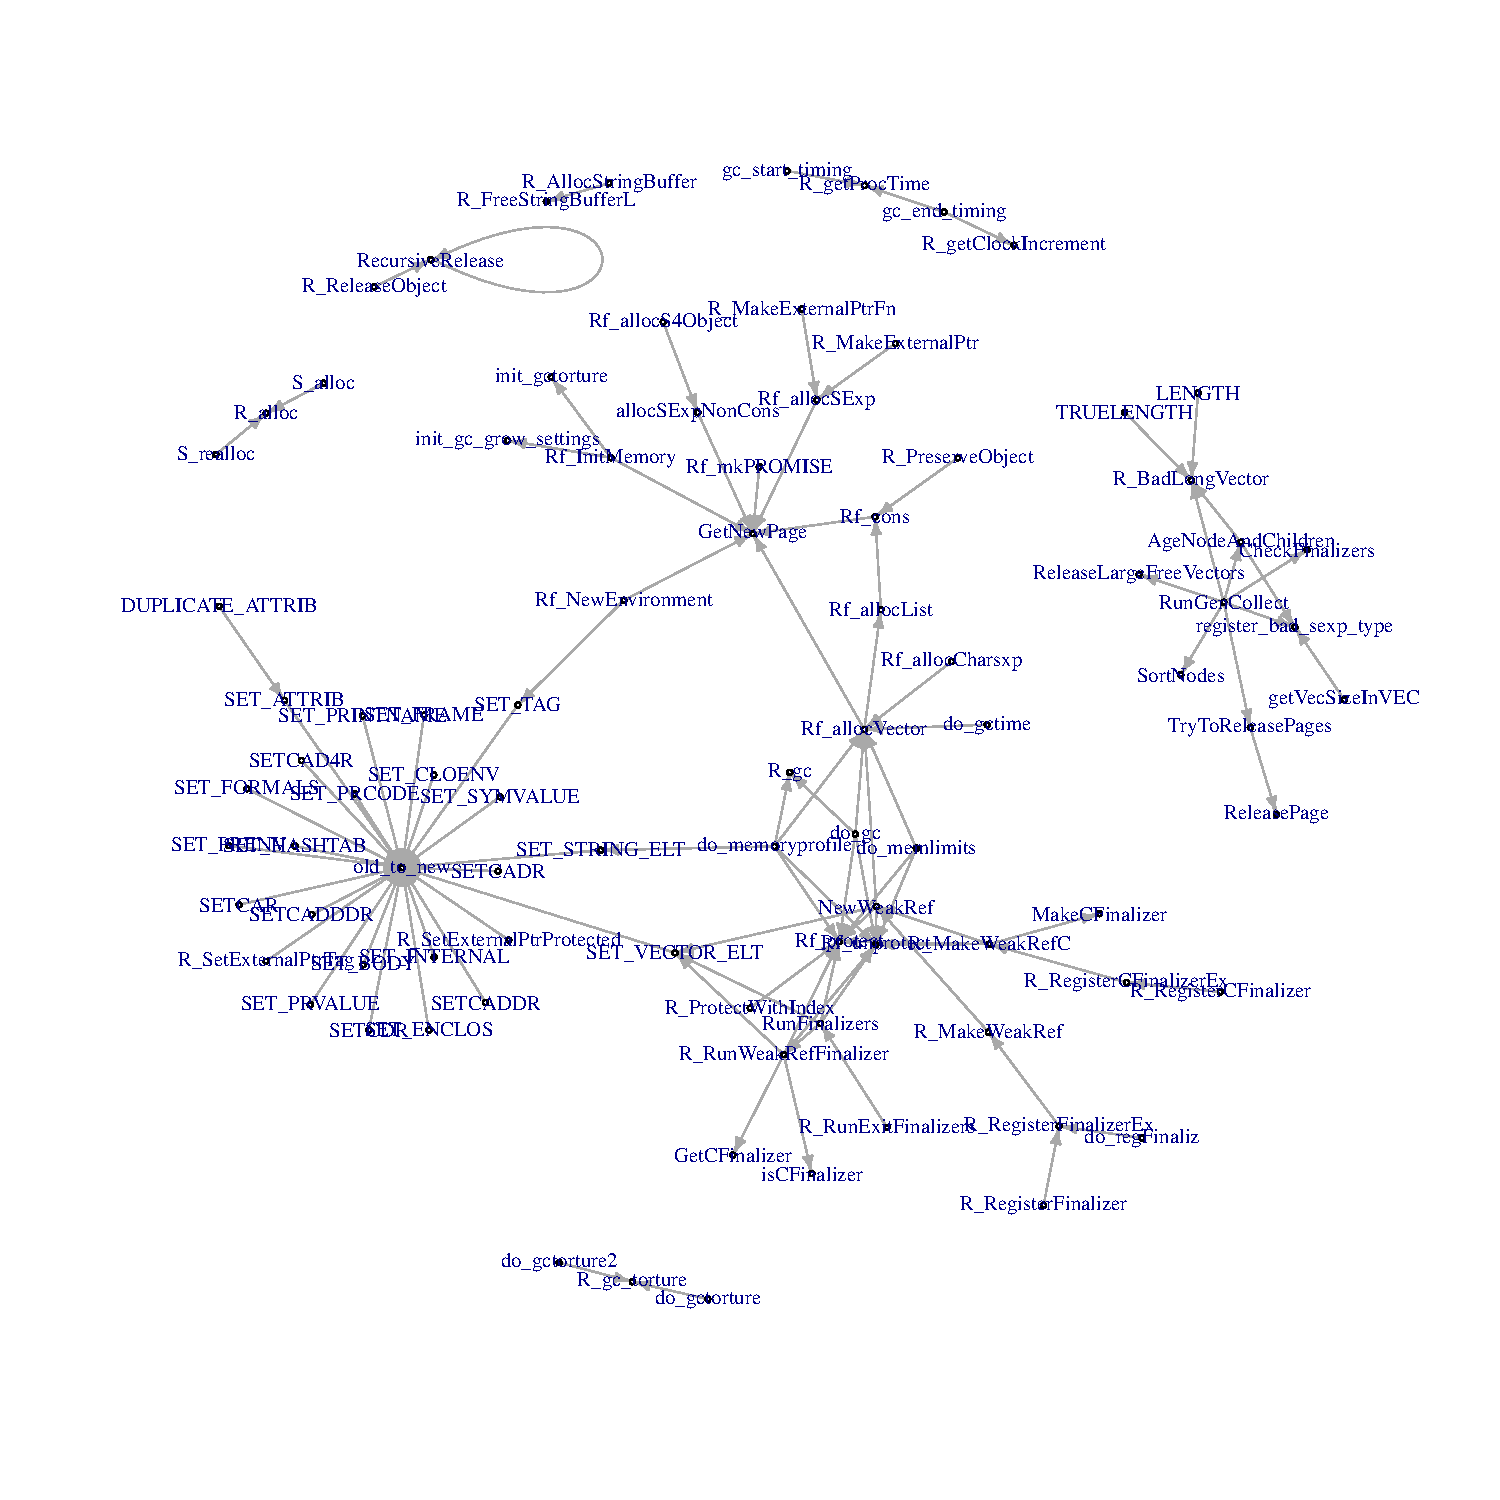
\includegraphics[width=\textwidth,height=.9\textheight]{callgraph.pdf}
\caption{A display of the call graph for the file \file{memory.c} in
  \R's source. This displays which routines call which other routines
  within that file alone. The clusters and important routines become evident.}
  \label{fig:callgraph}
\end{figure}

I have used the \Rpkg{findCalls} function when creating bindings to
third-party libraries to determine which routines currently have no
wrapper routine.


%\subsection[Registering R-callable routines]{Registering \R-callable routines}
\paragraph{Registering \R-callable routines}
We mentioned in section~\ref{sec:Introduction} registering native
routines we can call from \R{} via the \Rfunc{.C}, \Rfunc{.Call} and
\Rfunc{.External} interfaces.
The registration information is \C{} code that looks something like
\begin{CCode}
static R_CallMethodDef CallEntries[] = {
     {"R_csv_sample", (DL_FUNC) &R_csv_sample, 2},
     {NULL, NULL, 0}
};

void attribute_visible R_init_FastCSVSample(DllInfo *dll)
{
   R_registerRoutines(dll, NULL, CallEntries, NULL, NULL);
   R_useDynamicSymbols(dll, TRUE);
}  
\end{CCode}
This example comes from the \Rpkg{FastCSVSample} package
(\url{http://github.com/duncantl/FastCSVSample}). In this case, there
is only one \C{} routine we invoke via the \Rfunc{.Call} function.  In the
\Rpkg{stats} package, there are $83$ \Rfunc{.Call} and $10$ \Rfunc{.C}
routines, with registration information for all. 

It is tedious, and hence error-prone, to manually create this
registration information, and also to update it as the code evolves.
Instead, we can use the \Rfunc{createRegistrationCode} function to
generate it for us.  This is often as simple as something like
\begin{RCode}
rg = createRegistrationCode("~/GitWorkingArea/FastCSVSample/src")  
cat("#include <R_ext/Rdynload.h>", rg, sep = "\n", file = "init.c")
\end{RCode}
For an \R{} package, we specify the \dir{src} directory of that
package.  We can also provide arguments for the parser such as
\Rarg{includes} or pre-processor definitions via the \Rarg{args} parameter
using \Rfunc{createRegistrationCode}'s \Rarg{\dots} parameter.  The function processes each \C{} and \Cpp
file in the directory and determines which routines can be called via
the \Rfunc{.C} interface and which can be called by \Rfunc{.Call}.  It
does this by examining the signatures and determining which are
consistent with the two different call mechanisms.  It then creates the
registration information and also generates the \Cfunc{R_init_...}
routine, using the name of the package as suffix.

The \R{} registration mechanism doesn't currently permit the
programmer to specify which type of \R{} object is expected for each
parameter in a \Rfunc{.Call} routine, e.g., an integer or numeric
vector, or a function or a list.  The \Rpkg{RCIndex} functionality
does, however, allow us to infer this by analyzing the code within a
routine and determining how it is being accessed.  This could be added
to the registration information and allow \R{} to perform run-time
checks or coercion to the appropriate types in call to the routine.


\paragraph{Listing included files}
The function \Rfunc{getInclusions} allows us to obtain a list of all
the files included in our translation unit, both directly and
indirectly.  This allows us to find what files include other files,
which files are included by multiple files, what files are not included in a
directory and so on. We can also visualize the implicit network.
%XXX not well written - tidy up.


%XXX Some examples????


\subsection{Low-level building blocks}\label{sec:BuildingBlocks}

The functions we described above do not require the user to know any
of the details of \libclang{} and how \Rpkg{RCIndex} extracts the
information from a source code file.  To work with the results of some
of these functions, however, the \R{} programmer may need to know a
little about \libclang's type system. Furthermore, to go beyond these
functions and extract different information, a programmer needs to
understand the lower-level tools on which these functions were built.
At the very least, it is useful to know how to create a translation
unit directly rather than re-parsing the same file multiple times.  In
this section, we discuss the functionality for creating a translation
unit, working with cursor objects and cursor hierarchies.  We'll
address writing visitor functions after these topics.



\paragraph{Creating a translation unit} 
One of the two vital functions in \Rpkg{RCIndex} is \Rfunc{createTU}.
This takes the name of a source file and parses it into a translation
unit object in memory, returning a reference to that as an opaque \R{}
object.
The signature of the function is 
\begin{RCode}
createTU(src, includes = character(), 
         idx = createIndex(verbose = verbose), 
         args = character(), 
         verbose = getOption("ShowParserDiagnostics", TRUE), options = 0)   
\end{RCode}
The \Rarg{includes} parameter allows us to specify one or more paths
to directories in which to find \Ckeyword{\#include}'d header files. We
can pass arguments to control the parser via the \Rvar{args}
parameter. These can be pre-processor flags and definitions such as
\verb+-DHAVE_CONFIG_H+, or any of the options the \libclang{} parser
understands such as \texttt{-ferror-limit=1000} % \libclangFlag{-ferror-limit=1000} 
and
\mbox{\texttt{-fparse-all-comments}}. % \libclangFlag{-fparse-all-comments}.
The entire set of options is documented in
the \clang{} user manual
(\url{http://clang.llvm.org/docs/UsersManual.html})\footnote{The code
  generation options are not relevant as we are not generating code,
  only parsing it.}.

\Rfunc{createTU}'s \Rarg{options} parameter allows us specify certain additional
control options for creating the parser beyond the \Rarg{args} parameter.  These control
aspects such as skipping the bodies of routines when we just want the
declarations, keeping a more complete record of the pre-processing
steps, and other aspects that don't concern us.
We specify these options either as a combination of
bitwise-enumeration values from the \Rvar{CXTranslationUnit_Flags}
class.
For instance, to skip the body of the routines and to indicate the 
translation unit is incomplete, we can use
\begin{RCode}
CXTranslationUnit_SkipFunctionBodies | CXTranslationUnit_Incomplete  
\end{RCode}
These two \R{} variables represent these two options and we are
combining them via the \Rop{|} operator.
An alternative, but equivalent,  approach is to use short-hand names as a character
vector, e.g.,
\begin{RCode}
c("SkipFunctionBodies", "Incomplete")
\end{RCode}

The \Rarg{index} parameter for the \Rfunc{createTU} function is often
omitted as we typically parse a single source file and work on it
separately from others.  However, as we mentioned, routines often
refer to other routines or variables in other source files in the same
project.  The index is a container for related translation units and
provides the mechanism for resolving references across translation
units it manages.  Therefore, if we want to work on multiple related
source files, we should first create an index and then pass this to
each call to \Rfunc{createTU}, e.g.,
\begin{RCode}
index = createIndex()
tus = lapply(list.files("src", pattern = "\\.c$", full.names = TRUE),
               createTU, index = index)
\end{RCode}
%$
Alternatively, we can pass a vector of file names in the call to
\Rfunc{createTU} and it will create a translation unit for each, using
the same index and \Rarg{args} and \Rarg{includes}. So our example
could be  written as 
\begin{RCode}
tus = createTU(list.files("src", pattern = "\\.c$", full.names = TRUE))  
\end{RCode}
%$

When creating an index, we can control whether it displays errors,
warnings and general diagnostic information about the code on the
console.  We can disable this via the \Rarg{verbose} parameter and
passing \Rfalse{} as its value.

\paragraph{Working with cursors}
A translation unit is a container for the parse tree.
We can query the name of the source file  with
\Rfunc{getFileName}. More importantly, we can 
access the root cursor in a translation unit
with either of the following expressions
\begin{RCode}
as(tu, "CXCursor")
getTranslationUnitCursor(tu)
\end{RCode}
A cursor in \R{} has the class \Rclass{CXCursor}.

A cursor is a representation  of a general semantic concept such
as a call expression, a binary operation, a variable declaration and
so on.  We find out its particular kind or purpose using
the \Rfunc{getCursorKind}  function or the short-hand
\Rdollar{} operator. So the following are equivalent
\begin{RCode}
  getCursorKind(cur)
  cur$kind
\end{RCode}
%$

Most cursors have an associated string such as the name of the routine
being invoked in a call expression or a variable being referenced in a
variable declaration.  We get this string via the \Rfunc{getName} function.

We can retrieve the actual text from the source file associated with a
cursor using \Rfunc{getCursorTokens}. This is important in some cases
when the kind of the cursor doesn't give us enough detail to
disambiguate between various possibilities.  For example, a binary
operator doesn't tell us what operator was being used.  For this, we
look at the actual text. \Rfunc{getCursorTokens} conveniently returns
the associated source code text already broken into lexical tokens
with names that identify their token types, e.g., \dquote{Punctuation}.

If we parse the code using the \verb+-fparse-all-comments+ argument to
\Rfunc{createTU}, we can retrieve the comments associated with certain
kinds of cursors, i.e., variable, routine and type declarations.  There
are several functions to access the comment.  We can get the text with
\Rfunc{getRawCommentText}. We can also get a brief version of the
comment corresponding to certain conventions for marking up
documentation in comments via \Rfunc{getBriefComment}, i.e.,  the text
to the end of the line after a \verb+\brief+ directive in the comment.  The
\Rfunc{getParsedComment} function returns an actual \Rclass{CXComment} object
and we can treat this as a hierarchical object with child comments.

In some situations, it is important to map a cursor to its location in
the source file. \Rfunc{getLocation} returns the filename and the line
and column numbers and the number of bytes (or offset) from the start
of the file. \libclang{} has various concepts of location and we can
express which one we want to use by name, i.e., one of
\dquote{Expansion}, \dquote{Instantiation} and \dquote{Presumed}.

Some kinds of cursors are references to other elements in the
translation unit. For example, in a call expression, the routine being
called is represented by a reference cursor that refers to the actual
routine. We can resolve that reference with the
\Rfunc{getCursorReferenced} function.

Recall that cursors are recursive structures, often with child cursors.  We
typically write functions that traverse this tree using
\Rfunc{visitCursor} and we will discuss this in the next section.
However, it is convenient at times to explicitly access a cursor's
children, and their children and so on.  We can conceptually think of the
cursor as being like an \R{} list with the children as its
elements. This allows us to access the children individually using
\Rexpr{cur[[i]]}, where \Rvar{i} is the index of the child ( with the
first child at index 1). We can't use names to index the children or
the \Rdollar{} operator. We can find the number of children a
cursor has using the \Rfunc{length} function.  We can access the entire list of
children explicitly by calling the \Rfunc{children} function and this allows us to loop
over them with \Rfunc{lapply} or \Rfunc{sapply}.

In addition to being able to descend the cursor tree, we can navigate
up the hierarchy using \Rfunc{getCursorSemanticParent} and in a
slightly different sense of the hierarchy with \Rfunc{getCursorLexicalParent}.


\paragraph{Traversing a cursor tree}
To traverse a cursor tree, we typically use the \Rfunc{visitCursor} function.
This is (currently) more efficient than recursively processing the
entire tree with \R{} code looping over the children. However, writing
visitor functions can be complicated as it typically involves
maintaining state across calls to the same function. This is not very
common in \R{} so needs some discussion.


\subsection{Writing visitor functions}
%Closures, reference classes
%Reference class and inheritance.


%XXX Correct this to talk about traversing any cursor, not just the TU.
The primary way to extract information from a translation unit is to
use the \Rfunc{visitTU} function.  This takes the name of a source
file or an already parsed translation unit.  The second argument is a
``visitor'' function.  This can take various forms but
essentially correspnds to an \R{} function (or the address of a native
symbol).  \libclang{} iterates over some or all of the cursors in the
translation unit and calls the \R{} function for each each of these
cursors, passing it both the current cursor and its parent cursor, for
context.  The function can perform any computations it desires and
typically extracts and assigns any information it wants from each cursor, or the
cursor itself.
%XXXX
% Move this to after the closures and explain that we can always
% Recurse, but it can be a waste of time.


The visitor function typically stores information that persists across
the calls to it made by \libclang.  We then access these objects when
\libclang{} has completed traversing the tree.  While we may be
inclined to use global variables, e.g., in \R{}'s global environment or
interactive ``work space'', this is a bad idea.  Instead, we want to
use variables that are local to this particular visitor function.  We
can do this in two basic ways -- reference classes or closures, also
known as lexical scoping.  In fact, these two are very similar.

We'll focus on a very simple example which merely
iterates over the sub-cursors and finds the name and location of each
routine in the translation unit.  We are looking for cursors at the
top-level of the translation unit which have a cursor kind
\Rvar{CXCursors_FunctionDecl}.  We ignore any other cursors.

We will store the name of each routine and also its line number.
We have to put these into a non-local variable within a call to our
visitor  function and then be able to retrieve them. This is a closure.
Creating a closure is quite simple but requires understanding how \R{}
finds variables.  One approach to creating a closure is to define a
function that returns one or more functions.  We often call this a
generator function.
We can define our generator function something like
\begin{RCode}
genRoutineLocations = 
function() 
{
   locations = integer()

    visitor = function(cur, parent) {
       if(cur$kind == CXCursor_FunctionDecl) 
         locations[[ getName(cur) ]] <<- getLocation(cur)$location["line"]

        CXChildVisit_Continue
    }

    list(update = visitor, locations = function() locations)
}
\end{RCode}
There are several things to note.  Firstly, we have defined the
\Rfunc{genRoutineLocations} function. That is not what we will use to
traverse the tree. Instead, we call it to get a new pair of functions
returned in a list.  We will pass the \Rel{visitor} element of that
list to \Rfunc{visitCursor}.  Secondly, note the use of \verb+<<-+
when we assign the line number to the element of our \Rvar{locations}
vector. This is a non-local assignment an the updated value will
persist across calls to this function. Thirdly, note that the
\Rvar{locations} vector is defined in the body of
\Rvar{genRoutineLocations}, not within our visitor function. The
visitor function merely modifies it.  Fourthly, our second function in
the returned list (\Rel{locations}) is an anonymous function also
defined during a call to \Rfunc{genRoutineLocations} and it returns
the current value of the \Rvar{locations} variable when it is called.
This allows us to retrieve the results after they were added in the
different calls to our visitor function.  Lexical scoping and closures
are described in various texts about \R{} and \cite{bib:LexicalScoping}
is the definitive reference.

We can now use our generator function and obtain the line numbers of
the different routines. We do so with
\begin{RCode}
f = system.file("exampleCode", "fib.c", package = "RCIndex")
col = genRoutineLocations()
visitCursor(f, col$visitor)
col$locations()
\end{RCode}
Our call to \Rfunc{genRoutineLocations} returns the list of two
functions.  We pass the \Rel{visitor} element to \Rfunc{visitCursor},
along with the name of the source code file.  Then we retrieve the
updated contents with the second function \Rel{locations}.


As an aside, note that in this particular case, we don't need to
recursively descend through the cursors as the routines will all be
immediate children of the translation unit.  Therefore, our visitor
function returns \Rvar{CXChildVisit_Continue} to move to the next
sibling and not down across its children.  This saves times processing
irrelevant cursors.

Closures are very powerful but confuse some \R{} programmers.
Reference classes may be more familiar, especially to those familiar
with classes in \Cpp, \Java{} or \Python.  The idea is that we define
a class that has methods that share variables.  Our methods will be
our \Rel{visitor} and \Rel{locations} accessor functions in the generator
function above, and the fields or variables will be the
\Rvar{locations} numeric vector.  We can use the same code, but
aggregate it in a different way to define a reference class as:
\begin{RCode}
RoutineLocationVisitor =
setRefClass("RoutineLocationVisitor",
    fields = list(locations = "numeric"),
    methods = list(getLocations = function() 
                                     locations,
                   visitor = 
                       function(cur, parent) {
                         if(cur$kind == CXCursor_FunctionDecl) 
                            locations[[ getName(cur) ]] <<- 
                                   getLocation(cur)$location["line"]
                               
                         CXChildVisit_Continue
                       }))
\end{RCode}
Here, we explicitly identify the shared variable and the methods via
the \Rarg{fields} and \Rarg{methods} parameters.  The only real
difference between this and our generator function is that we have
to call our accessor function to retrieve the \Rvar{locations} value
\Rfunc{getLocations} rather than \Rfunc{locations}.  This is merely to
avoid have a field and a method with the same name.

We can now use this reference class in almost exactly the same way we
used our  generator function:
\begin{RCode}
col = RoutineLocationVisitor()
visitCursor(f, col$visitor)
col$getLocations()
\end{RCode}
The \Rfunc{RoutineLocationVisitor} function returned by
\Rfunc{setRefClass} creates a new instance of this reference class.
We pass the \Rfunc{visitor} method to \Rfunc{visitCursor} and then
call the function \Rfunc{getLocations} to obtain the results.



You can use any reference class you want and then pass the visitor or
update method to \Rfunc{visitTU}.  However, it can be convenient to
define your reference class to extend the \Rclass{RefCursorVisitor} class in
the \Rpkg{RCIndex} package. This allows you to pass the entire
reference object to \Rfunc{visitTU} and to get the results back
directly. This is merely syntactic sugar to simplify the
programming. It changes the code above to create the reference class,
call \Rfunc{visitCursor} and retrieve the results to the more succinct
\begin{RCode}
visitCursor(cur, RoutineLocationVisitor)
\end{RCode}
Essentially, extending the \Rclass{RefCursorVisitor} class allows
\Rfunc{visitCursor} to identify the visitor and the result functions.
The only change we need to make when defining our reference class
is to add the \Rarg{contains} argument in the call to
\Rfunc{setRefClass}, i.e.,
\begin{RCode}
setRefClass("RoutineLocationVisitor",
            contains = "RefCursorVisitor",
            fields = list(locations = "numeric"),
            methods = list(getLocations = function() locations,
                       .....))
\end{RCode}



Similar to the \Rclass{RefCursorVisitor} reference class, we can use
an S4 class -- \Rclass{S4CursorVisitor} -- to combine the visitor and
result function and pass the two together to \Rfunc{visitCursor}.  We
typically create our two functions as before via a generator function,
and then combine the two functions into a formal object with, for
example,
\begin{RCode}
col = genCollector()
visitCursor( cur, new("S4CursorVisitor",  update = col$update, result = col$vars))
\end{RCode}
Again, the purpose of this \Rclass{S4CursorVisitor} class is merely to
allow \Rfunc{visitCursor} to identify the two functions -- the visitor
function and the function to access the results.


\paragraph{Copying cursors}
The \Rfunc{visitCursor} function, by default, makes a copy of each of
the \C-level cursor objects in each call to our visitor function.
This, combined with the garbage collection mechanism in the package,
ensures that if the visitor function assigns a cursor to a non-local
variable so it persists after that specific call, it will remain
valid.  If the visitor function does not need the cursors after each
call, it can avoid this unnecessary copying.  We do this by passing
\Rfalse{} for the value of the \Rarg{clone} parameter of the
\Rfunc{visitCursor} function.  If the visitor function wants to store
a cursor, it can explicitly copy the cursor itself by calling the
\Rfunc{clone} function and assigning the new cursor to a non-local
variable.  Generally, it is safest to use the defaults and incur the
slight overhead of cloning.


\paragraph{Controlling how \libclang{} traverses the tree}
By default, \Rfunc{visitCursor} will arrange for the visitor function
to be called for each cursor in the cursor hierarchy.  Sometimes we
don't need to see very cursor, but perhaps just the top-level cursors
of the translation unit or the parameters in a routine, but not its
body.  A visitor function can indicate to \libclang{} whether to
recursively process the sub-curors of the current cursor being
visited, or to skip the entire sub-hierarchy and move to the next
sibling of the current cursor.  Alternatively, a visitor function may
determine that it has seen enough and doesn't need to process any more
cursors, i.e., gracefully terminate the traversal of the tree.  To do
this, the visitor function returns any of \Rvar{CXChildVisit_Recurse},
\Rvar{CXChildVisit_Continue} or \Rvar{CXChildVisit_Break}.  The
visitor function can return a different value on each invocation and
so dynamically determine where to visit next.  

As an example of controlling the traversal, consider that we want to
process all of the nodes in a particular routine named \Cfunc{bar} but
no other routines or elements of the translation unit. 
We could define our visitor function something like
\begin{RCode}
genVisitor = 
function()
{  
    inBar = FALSE
    
    update =
      function(cur, parent) {
        if(cur$kind == CXCursor_FunctionDecl) {
          if(inBar) {
            cat("quitting having reached the routine", getName(cur), "\n") 
            return(CXChildVisit_Break)
          }
          
          if(getName(cur) == "bar") {
            inBar <<- TRUE
            return(CXChildVisit_Recurse)
          } else
            return(CXChildVisit_Continue)
        } else {
             # processing the cursors within the bar routine.
          print(cur$kind)
          return(CXChildVisit_Recurse)
        }
      }
}
\end{RCode}
%$
We can then invoke it with
\begin{RCode}
f = system.file("exampleCode", "mutateArg.c", package = "RCIndex")
visitTU(f, genVisitor())  
\end{RCode}
We keep a non-local variable state variable to see if we have
already encountered the routine \Cfunc{bar}.
If we have and we see another routine, we terminate the traversal.
If we see a routine that isn't bar, we skip to the next routine
with \Rvar{CXChildVisit_Continue}.
If the routine is named \Cfunc{bar}, we tell \libclang{}
to process the sub-cursors.




\section{Extended Examples and Applications}\label{sec:Examples}
In this section, we explore some more advanced examples of how to use
the \Rpkg{RCIndex} package to get different information from a
translation unit.  One of the best sources of such examples is the set
of high-level functions in the package itself,
e.g., \Rfunc{getRoutines}, \Rfunc{getCppClasses}.  In the package and
in the example in this section, we have used the generator function
and lexical scoping approach to implement a set of collector functions
that gather the different types of information we want.

In section~\ref{sec:Introduction}, we provided numerous motivating
applications of being able to process native code.  We will present
partial/heuristic approaches to some of these.  One aim of these
examples is to illustrate how to traverse the translation unit and
sub-cursors and work on the structure of the information.  Another aim
is to illustrate how to work with \libclang's type system.

\subsection[Checking for garbage collection errors in native code for R]{Checking for garbage collection errors in native code for \R{}}
In this example, we will write code that can examine a \C{} routine
written to be called via \R's \Rfunc{.Call} interface and try to
identify if there are possible errors related to ensuring \R{} objects
are not garbage collected prematurely.  The \R{} API uses the macros
\Cfunc{PROTECT} and \Cfunc{UNPROTECT} to mark an object as being in
use and stop if from being garbage collected and to unmark a number of
protected objects.  For example, the \C{} code in
figure~\ref{fig:ProtectCorrect} creates two new \R{} objects and
protects them both, performs some computations that populate the
objects and then unprotects both with a call \Cexpr{UNPROTECT(2)}.  In
contrast, the code in figure~\ref{fig:ProtectIncorrect} does not
protect the \R{} object it creates.  It is quite possible that after
allocating \Cvar{ans}, \R{} will release that object when it allocates
\Cvar{names} in the next expression. At that point, the memory is
corrupted and errors and crashes are likely.
In other cases, we might protect the \R{} objects we create,
but fail to unprotect them, or at least some of them.

\noindent
\begin{figure}[ht]
\begin{minipage}[t]{0.45\linewidth}
\centering
\begin{CCode}
SEXP
R_foo_correct(SEXP r_x)
{
  SEXP ans, names;
  int n = Rf_length(r_x);
  double *x = REAL(x);
  PROTECT(ans = NEW_NUMERIC(n));
  PROTECT(names = NEW_CHARACTER(n));
  for(int i = 0; i < n; i++) {
    char *str;
    REAL(ans)[i] = foo(x[i], &str);
    SET_STRING_ELT(names, i, 
                     mkChar(str));
  }
  SET_NAMES(ans, names);
  UNPROTECT(2);
  return(ans);
}
\end{CCode}
\caption{This is a simple and correct \C{} routine
that protects and unprotects the \R{} objects it creates.}
\label{fig:ProtectCorrect}
\end{minipage}
\hspace{0.5cm}
\begin{minipage}[t]{0.45\linewidth}
\centering
\begin{CCode}
SEXP
R_foo_incorrect(SEXP r_x)
{
  SEXP ans, names;
  int n = Rf_length(r_x);
  double *x = REAL(x);
  ans = NEW_NUMERIC(n);
  names = NEW_CHARACTER(n);
  for(int i = 0; i < n; i++) {
    char *str;
    REAL(ans)[i] = foo(x[i], &str);
    SET_STRING_ELT(names, i, 
                       mkChar(str));
  }
  SET_NAMES(ans, names);
  return(ans);
}

\end{CCode}
\caption{This version does not protect the \R{} objects and, hence,
  also  doesn't unprotect them.}
\label{fig:ProtectIncorrect}
\end{minipage}
\end{figure}


%XXX Clean this up wrt. to macro expansions. Ignore them  but just
%mention it is possible.
We will develop an \R{} function that will attempt to check for common
problems related to garbage collection.  Our function take the
\libclang{} cursor for a routine and will then traverse the
nodes/cursors throughout that tree. It will find calls to known
routines that alloc \R{} objects (specifically \Cfunc{Rf_allocVector})
and also calls to \Cfunc{Rf_protect} and \Cfunc{Rf_unprotect}.  At its
very simplest, we can count the number of allocations, the number of
calls to \Cfunc{Rf_protect} and attempt to determine the value passed
to \Cfunc{Rf_unprotect}.  If these don't match, we can indicate a
potential error.  This is a simple heuristic approach, but it may
catch some cases.

What about \Cfunc{NEW_NUMERIC}, \Cfunc{PROTECT} and \Cfunc{UNPROTECT}?
In some cases, these are acutally pre-processor macros and in others
they are actually routines. They expand to
\Cexpr{Rf_allocVector(REALSXP, n)} and calls to \Cfunc{Rf_protect} and
\Cfunc{Rf_unprotect}.  We can find these expansions and substitutions
in the translation unit. Alternatively, we can use our knowledge of
how the \R{} API works.


Since we will traverse over the sub-cursors, we need a visitor
function. We'll use a closure, but again, we could use a reference
class.  We need variables in which we can record the number of calls
to each of \Cfunc{Rf_allocVector}, \Cfunc{R_protect} and
\Cfunc{R_unprotect}.  We'll call these variables \Rvar{numAllocs},
\Rvar{numProtectCalls} and \Rvar{numUnprotectCalls}, respectively.
For the first two routines, we just increment the current value
in the corresponding \R{} variable.
For \Cfunc{Rf_unprotect}, we'll collect the argument for each call to
\Cfunc{Rf_unprotect}. This might be a literal value, e.g. $2$ in our
example, or a variable or a general expression.

We have now identified the basic strategy for our visitor function.
Next, we need to specify the details for the different types of
cursors we encounter. A call to any of our routines will be identified
by a cursor with a kind \Rvar{CXCursor_CallExpr}.  We can get the name
of the routine being called using \Rfunc{getName} applied to this
cursor. (There are other ways also, but this is the simplest.)  Based
on this name, we update the relevant counter or ignore the call.  If
the call is to \Cfunc{Rf_unprotect}, we have to arrange to get its
argument.  We can use either of two approaches for this.  We can set a
flag in our closure to indicate we are processing the sub-cursors of a
\Cfunc{Rf_unprotect} call and then subsequent calls to our visitor
function can check this and interpret the sub-cursors
appropriately. Alternatively, we can explicitly traverse the children
of the current call cursor to determine the argument.
We'll use the former approach.

We define our generator  function as
\begin{RCode}
genProtectAnalyzer =
function()
{
  numAllocs = 0  
  numProtectCalls = 0
  numUnprotectCalls = numeric()

  inUnprotect = FALSE  
  allocCounterVarName = ""    
  unProtectParent = NULL

  update = function(cur, parent)    {
    k = cur$kind

    if(inUnprotect && identical(unProtectParent, cur) ) {
       unProtectParent <<- NULL
       inUnprotect <<- FALSE
     }
    
   if(k == CXCursor_CallExpr) {
      fn = getName(cur)
      print(fn)
      if(fn == "PROTECT" || fn == "Rf_protect")
        numProtectCalls <<- numProtectCalls + 1
      else if(fn == "UNPROTECT" || fn == "Rf_unprotect") {
        numUnprotectCalls <<- numUnprotectCalls
        unProtectParent <<- parent
        inUnprotect <<- TRUE
      } else if(fn %in% c("Rf_allocVector", "NEW_NUMERIC", "NEW_INTEGER", "NEW_LOGICAL", "NEW_CHARACTER"))
          numAllocs <<- numAllocs + 1
    } else if(inUnprotect) {
       if(k == CXCursor_IntegerLiteral) {
          val = getCursorTokens(cur)["Literal"]
          numUnprotectCalls <<-  c(numUnprotectCalls, as.integer(val))
       } else if(k == CXCursor_FirstExpr) {
           allocCounterVarName <<- getName(cur)
       }
    }
    
    CXChildVisit_Recurse
  }

  list(update = update,
       info = function() {
                 list(numProtectCalls = numProtectCalls,
                      numUnprotectCalls = numUnprotectCalls,
                      inUnprotect = inUnprotect,
                      numAllocs = numAllocs)})
\end{RCode}
%$
For the present, ignore that second expression
in our visitor function, the \Rfunc{if} expression.
We'll discuss this below.



Before we can check the routine, we have to read it into \R{}.
We can do this with \Rfunc{getRoutines} via
\begin{RCode}
f = system.file("exampleCode", "protectIncorrect.c", package = "RCIndex")
r = getRoutines(f, f, includes = sprintf("%s/include", R.home()))
\end{RCode}
Note that we specified the include directories so that
the parser could find \file{Rinternals.h} and the other 
\R{} header files.

We create our visitor function by calling the generator function
and then we pass the visitor to \Rfunc{visitCursor},
along with our routine we want to check:
\begin{RCode}
v = genProtectAnalyzer()
visitCursor(r$R_foo_incorrect, v$update)
v$info()
\end{RCode}
The output is 
\begin{ROutput}
$numProtectCalls
[1] 0

$numUnprotectCalls
numeric(0)

$numAllocs
[1] 2
\end{ROutput}
We can see there are two allocations and no calls to protect or
unprotect.  
In constrast, when we run this on the correct version, 
each of the three counts has a value of $2$.

\begin{comment}
f = system.file("exampleCode", "protectCorrect.c", package = "RCIndex")
r = getRoutines(f, f, includes = sprintf("%s/include", R.home()))
v = genProtectAnalyzer()
visitCursor(r$R_foo, v$update)
v$info()
\end{comment}
%$

We should revisit the \Rfunc{if} expression near the beginning
of our visitor function:
\begin{RCode}
if(inUnprotect && identical(unProtectParent, cur) ) {
   unProtectParent <<- NULL
   inUnprotect <<- FALSE
}
\end{RCode}
The purpose of this is to ensure that we don't continue to collect
information from other cursors after we have processed any call to
\Cfunc{UNPROTECT}.  If we didn't have this, the variable
\Rvar{inUnprotect} would remain \Rtrue.  As a result, if there are
\C{} expressions in the body of the routine after the call to
\Cfunc{UNPROTECT} and they contain literal values or
\Rvar{CXCursor_FirstExpr} cursors, we will continue to accumulate
these as if they related to the \Cfunc{UNPROTECT} call.  As a result,
we need to determine when we have finished examining the sub-cursors
of the \Cfunc{UNPROTECT} call.  To do this, we record the parent
cursor of the \Cfunc{UNPROTECT} call in \Rvar{unProtectParent}. Each
time our visitor is called, we can compare the current cursor to this
cursor and if they are the same, we are back to a sibling of the
\Cfunc{UNPROTECT} call.

Setting and unsetting a state variable across calls to a visitor
function can be complex and often requires clear thinking.
We could have used the other approach which was to detect
the call to \Cfunc{UNPROTECT} and immediately determine its arguments
using \Rfunc{children}. For example, we could have added the code
\begin{RCode}
arg = children(cur)[[2]]
if(arg$kind == CXCursor_IntegerLiteral)
   as.integer(getCursorTokens(arg)["Literal"])
\end{RCode}
%$
This makes the visitor function a great deal simpler and also slightly
faster as we can avoid traversing the sub-cursors again.  However,
sometimes we have to use state, in particular when the information we
need to extract is not in sub-cursors but in silbing cursors and their
descendants.


As a final remark about this example, we could make this more general
and sophisticated.  A reasonably common idiom is to use a variable to
count the number of calls to \Cfunc{PROTECT} we make, incrementing it
each time. Then we pass this to \Cfunc{UNPROTECT}, e.g.
\begin{CCode}
 int n = 0;
 PROTECT(a = Rf_allocVector(...)); n++;
 PROTECT(b = Rf_allocVector(...)); n++;
 PROTECT(c = Rf_allocVector(...)); n++;
 PROTECT(d = Rf_allocVector(...)); n++;

 UNPROTECT(n);
\end{CCode}
 It is easy to omit incrementing the counter in one
or more cases. We can try to trace this by identifying the variable in
the call to \Cfunc{UNPROTECT} and then finding out where it is
incremented and try to find cases where it is not.
% Show example code




\subsection{Finding the signature for a foreign function interface call}\label{sec:RffiEG}

In this example, we focus on working with types in \Rpkg{RCIndex}.

As I mentioned in section~\ref{sec:Introduction}, there are two
packages (\Rpkg{Rffi} and \Rpkg{rdyncall}) that allow us to
dynamically invoke arbitrary native routines within an \R{} session
without having to write or compile any additional wrapper code.  Both
require a description of the signature of the routine to be
called. That is, we need the return type and the number and types of
the parameters.  We don't want the user to have to know or specify the
signature, so we want to be able compute it for them.  \Rpkg{rdyncall}
uses GCC-XML to get the information about the routines and generate
the corresponding signatures.  Here we'll show how to do it with
\Rpkg{RCIndex} and directly from the results of \Rfunc{getRoutines}
applied to the source code describing the routine(s) of interest.

Consider the simple  routine
\begin{CCode}
#include <math.h>
int
square_sin(int *val, int len, double *ans)
{
    int i;
    for(i = 0; i < len ; i++) {
	double tmp = sin(val[i]);
	ans[i] = tmp * tmp;
    }
    return(len);
}
\end{CCode}
This takes a vector of integer values and computes the
square of the sin of each element and returns the values
in the array of \Ctype{double} values. It returns the number
of elements it processed.

We'll look at how we can invoke this routine from \R{} using
\Rpkg{rdyncall} and then how we can generate the appropriate signature
programmatically.  Basically, before we can invoke the routine, we
have to compile the \C{} code into a shared
library, load that into \R{} and find the address of the symbol
\Cfunc{square_sin}.  We do this with a shell command
\begin{ShCode}
R CMD SHLIB rffi.c
\end{ShCode}
and the \R{} code
\begin{RCode}
dyn.load("rffi.so")
sym = getNativeSymbolInfo("square_sin")$address
\end{RCode}
%$

Next, we'll create some sample inputs:
\begin{RCode}
x = 1:10
ans = numeric(length(x))
\end{RCode}

To invoke the routine, we use the function \Rfunc{.rdyncall} function
in the \Rpkg{rdyncall} package. 
The call is 
\begin{RCode}
v = .dyncall(sym, "*ii*d)i", x, length(x), ans)
\end{RCode}
\Rfunc{.dyncall} takes care of marshalling the inputs and outputs
between \R{} and the native code.

The strange (and unaesthetic) string \verb+"*ii*d)i"+ is the
description of the signature of the routine.  It indicates that the
first argument (\verb+*i+) is a pointer to one or more \Ctype{int}
values, the second (\verb+i+) is a simple \Ctype{int} value specifying
the number of elements in the first argument, and the third
(\verb+*d+) is a pointer to one or more \Ctype{double} values.  The
\verb+)+ character separates the inputs from the return type and the
latter in this case is \verb+i+ and so an \Ctype{int}.  Of course, we knew this signature
by looking at the code, althought we didn't know the actual form it
took for \Rpkg{rdyncall}.

We'll write a function that uses \libclang{} and \Rpkg{RCIndex} to
create the signature for an arbitrary routine.  We'll assume our
function is passed a \Rclass{FunctionDecl} object returned by
\Rfunc{getRoutines}.  Recall that this contains the parameters and the
return type.  We can easily generate the signature with something
like
\begin{RCode}
makeSig = 
function(r)
{
   args = sapply(r@params, makeType)
   rtype = makeType(r@returnType)
   paste0( paste(args, collapse = ""), rtype)
}
\end{RCode}
The important part of this function is the call to \Rfunc{makeType}
for each type in the signature and that is the function we must implement next.
The \Rfunc{makeType} function is passed  either a \Rclass{CXCursor} or a \Rclass{CXType}.
We want to deal with the \Rclass{CXType} so must convert a
\Rclass{CXCursor} first. (We could of course use S3 or S4 methods to
do this also.)
\begin{RCode}
   if(is(ty, "CXCursor"))
     ty = getType(ty)
\end{RCode}
Once we have the \Rclass{CXType}, we can query the kind of type it is
with \Rfunc{getTypeKind}.
Given the kind, we first check to see if it corresponds to one of the
primitive \C{} types. We make a list of these by combining
the different enumeration values for \Rclass{CXType}, e.g.,
\Rvar{CXType_Double}, \Rvar{CXType_Int} and so on.
We can do this with
\begin{RCode}
BasicKinds = CXTypeKind[3:24]
\end{RCode}
since the primitive kinds are ordered contiguously in the
enumeration.

If the type does correspond to a basic type, we map it to 
the string that \Rfunc{.rdyncall} expects for this type.
These are listed in a table in the help page for \Rfunc{.rdyncall}.
\dquote{i} corresonds to \Rvar{CXType_Int}, \dquote{I} corresponds
to \Rvar{CXType_UInt} for an unsigned integer, and so on.
We express this map via the named \R{} vector
\begin{RCode}
rdyncallMap = c(
  v = CXType_Void,
  B = CXType_Bool,
  C = CXType_Char_U,
  C = CXType_UChar,
  c = CXType_Char32,
  c = CXType_Char_S,
  S = CXType_UShort,
  I = CXType_UInt,
  J = CXType_ULong,
  L = CXType_ULongLong,
  s = CXType_Short,
  i = CXType_Int,
  l = CXType_Long,
  l = CXType_LongLong,
  f = CXType_Float,
  d = CXType_Double
)
\end{RCode}
The value in the vector is the \libclang{} type kind. The
corresponding name is the \Rpkg{rdyncall} type identifier.
We can match the \libclang{} kind to the values in the vector and then
return the name of the corresponding element.
We do this with the simple function
\begin{RCode}
mapBasicKindToRdyncall =
function(kind)
{
  i = match(kind, rdyncallMap)
  if(is.na(i))
    stop("don't recognize that type")

  names(rdyncallMap)[i]
}
\end{RCode}
  
If the type kind of the type passed to \Rfunc{makeType} is not a basic
type, we have to examine it further.  We can compare the kind to
\Rvar{CXType_Pointer} to determine if it is a pointer, or call
\Rfunc{isPointerType} with the actual type object.  If the type is a
pointer type, we can get the type of element it points to with
\Rfunc{getPointeeType}.  Here we have to treat the \C{} string type
\Cexpr{char *} specially since \Rpkg{rdyncall} does.  We check if the
pointee type is of kind \Rvar{CXType_Char_S} and if it is, we return
the \Rpkg{rdyncall} string \dquote{Z}.

If the pointee type is not a \Rvar{CXType_Char_S}, then we check to
see if it is a basic type again. If so, we will combine the type
string for this basic type with a $\ast$ prefix, e.g., \dquote{*i}.  If
the type is not a basic type, then it is a pointer to a generic \C{}
type and we return \dquote{p}, as \Rpkg{rdyncall} requires.

We also have to deal with types that are not simply basic or pointer
types. For example, we may have a type declaration such as
\begin{CCode}
typedef long VecSize;
\end{CCode}
This is simply an alias or a new name for an existing type.
\Rpkg{rdyncall} doesn't care about the name, but only the actual type.
To deal with this in \Rpkg{RCIndex}, we can
use the canonical type to get at the actual type of the alias 
and pass this to a call to \Rfunc{makeType}.

The entire \Rfunc{makeType} function is defined as
\begin{RCode}
makeType = 
function(ty)
{
   if(is(ty, "CXCursor"))
     ty = getType(ty)

   kind = getTypeKind(ty) # or ty$kind
   
   if(kind %in% BasicKinds) {
     
      mapBasicKindToRdyncall(kind)

   } else if(kind == CXType_Pointer) {
     
     pty = getPointeeType(ty)
     if(getTypeKind(pty) == c(CXType_Char_S))
        "Z"
     else if((pk <- getTypeKind(pty)) %in% BasicKinds)
        sprintf("*%s", mapBasicKindToRdyncall(pk))
     else
        "p"
    
   } else if(kind == CXType_Typedef) {
     makeType(getCanonicalType(ty))
   }
}
\end{RCode}
%$

With the function defined, we can use it on
the routines in  \file{rffi.c}:
\begin{RCode}
r = getRoutines(system.file("exampleCode", "rffi.c", package = "RCIndex"))
sapply(r, makeSig)
\end{RCode}
\begin{ROutput}
square_sin    string1    string2   typedefn 
 "*ii*d)i"      "Z)v"      "Z)v"      "l)v" 
\end{ROutput}
These correspond to the declarations
\begin{CCode}
int square_sin(int *val, int len, double *ans);
void string1(char *x);
void string2(const char *x);
void typedefn(VecSize s)
\end{CCode}
The final signature illustrates mapping our
\Ckeyword{typedef} example to the  \Rpkg{rdyncall} string \dquote{l}
corresponding to a \Ctype{long}.

%We can identify whether a parameter is identified as being immutable.
%This allows us to avoid copying the argument before we pass it to
%the native routine.

We could go further with generating descriptions for use with
\Rpkg{rdyncall} or \Rpkg{Rffi} to process \Ckeyword{struct} and
\Ckeyword{union} types and \Cpp{} classes and so on.



\subsection{Determining unmodified inputs to a routine}\label{sec:MutabilityEg}

We mentioned in section~\ref{sec:Introduction} that it is can be
useful to determine if a routine modifies the memory pointed to by its
arguments.  Ideally, programmers would qualify parameters with a
\Ckeyword{const} declaration to indicate that it is not
modified. However, when this is not provided we do not know if it was
omitted or if the routine does actually change a parameter.
If we knew that it did not, we could avoid making a copy
of the inputs before calling it. 
In this example, we will build a simple-minded mechanism to try to
determine which parameters are modified within a routine.

%Similarly, if we could determine
%whether the routine allocated memory or expected to be allocated
%by the caller, we 

\noindent
\begin{figure}[ht]
\begin{minipage}[t]{0.45\linewidth}
\centering
\begin{CCode}
int
foo(int *x, int len)
{
    for(int i = 0; i < len; i++)
	x[i] = 2*x[i];
    return(len);
}

\end{CCode}
\caption{This routine modifies the memory pointed to by its
\Carg{x} argument.}
\label{fig:Mutability1}
\end{minipage}
\hspace{0.5cm}
\begin{minipage}[t]{0.45\linewidth}
\centering
\begin{CCode}
int
bar(int *x, int len)
{
    int total = 0;
    for(int i = 0; i < len; i++)
	total = 2*x[i];
    return(total);
}
\end{CCode}
\caption{Like \Cfunc{foo} on the left, this routine also 
expects a pointer to a \Ctype{int}, but it does not modify 
the contents of the memory pointed to by the argument.}
\label{fig:Mutability2}
\end{minipage}
\end{figure}

In this example, we show an alternative approach to traversing nodes
in the tree. We use a visitor but within the visitor explicitly
subset the children and their children with a single function call.

Consider the two routines in
figures~\ref{fig:Mutability1}~and~\ref{fig:Mutability2}.  Both take a
pointer to a collection of \Ckeyword{int} values.  The first changes
each element of the array. The second merely reads the elements of the
array. From the declaration, we cannot tell the difference.  We will
write a visitor function that traverses the code of the routine and
identifies expressions which modify one of the (pointer) parameters.
For simplicity, we will identify the names of the parameters of
interest, however, our function could compute the parameters as it
traverses the entire tree for the routine.  We'll start with a simple
visitor function, defined in a generator function to create the
closure. We can define this as 
\begin{RCode}
update =
function(cur, parent)  {
  k = cur$kind
  if(k == CXCursor_BinaryOperator && "=" %in% (toks <- getCursorTokens(cur)) ) 
      processLHS(cur[[1]])

  CXChildVisit_Recurse
}
\end{RCode}
%$

The basic strategy is that for each cursor, we determine if it is an
assignment operator. There is no simple function to do this in the
\libclang{} API, but we can combine different pieces of information to
get the answer. We check the kind of the cursor is
\Rvar{CXCursor_BinaryOperator} and then use \Rfunc{getCursorTokens} to
find the actual operator as a token.  If it is a \dquote{=}, we have
indentified our condition.  Using cursor tokens is a little less
precise than querying a specific cursor. The tokens may include
additional text before and after our cursor that may be misleading.

Once we have a binary operator, we are interested in its left-hand
side, i.e. the first child.  Rather than setting a state variable and
continuing to traverse the sub-cursors, we will explicitly process
this first child. We may have to traverse its children, but we will do
that with a separate visitor function -- \Rfunc{processLHS}.  This may
make the computations a little simpler.  So in our top-level visitor,
we access the first child of the current cursor with \Rexpr{cur[[1]]}
and  then call the function that will determine what is being modified.

Our next task is to define the \Rfunc{processLHS} function.  We could
define another visitor function, but instead we will manually traverse
the cursor tree.  We have various different situations to consider.
This left-hand side can be arbitrary \C{} code. Examples of the entire
expression include
\begin{CCode}
x[i] = 2*x[i];
total = 2*x[i];
*(x + i) = 2*x[i];  
y[ x[i] ] = 2*x[i];
*addr(y, x, i) = 2*x[i];
y[ f(x, i, y) ] = 2*x[i];
\end{CCode}
These illustrate assigning to an element, a variable,
a unary operator indexing \Cvar{x}, nested subsetting, 
calling a routine to get an address, and subsetting
with the index determined by a call to a routine.
The last two of these call other routines and we would have
to analyze their code to determine what is being modified.

We'll focus on the first four examples above.  We define a function
that can handle each of these different casesm.  \Rfunc{processLHS}
will be called with the cursor corresponding to the left-hand side of
the assignment.  We check to see if this is an array subscript
(\verb+[+), a variable reference (\verb+total+), a unary operator
(\verb+*+), another binary operator (\verb|x+i|), a call expression
(\verb+f(x, i, y)+ or \verb+addr(y,x, i)+) and so on.
The function is defined as
\begin{RCode}
processLHS = 
function(cur) {
  k = cur$kind

  id = if(k == CXCursor_ArraySubscriptExpr) { # x[i], y[x[i]], x[foo()]
         processLHS(cur[[2]])
         getName(cur[[1]])
       } else if(k == CXCursor_UnaryOperator){
         if(cur[[1]]$kind == CXCursor_ParenExpr)
           return(processLHS(cur[[1]][[1]]))
         else if(cur[[1]]$kind == CXCursor_DeclRefExpr)
           getName(cur[[1]])
         else if(cur[[1]]$kind == CXCursor_CallExpr)
             calls <<- c(calls, getName(cur[[1]]))
       } else if(k == CXCursor_FirstExpr || k == CXCursor_DeclRefExpr) {  
           # recursively from *( x + i) with x and again with i
         getName(cur)
       } else if(k == CXCursor_BinaryOperator) { # x + i arising in *(x + i)
         return(sapply(children(cur), processLHS))
       } else if(k == CXCursor_CallExpr)
             return(calls <<- c(calls, getName(cur)))
  
  if(!is.null(id) && id %in% paramNames)
      modifiedVars <<- c(modifiedVars, id)
} 
\end{RCode}
This function does ``visit'' the child cursors. Instead, it actively
extracts and processes them without returning control to the
\libclang{} iterator. This makes the logic a little easier to
understand.

Note that this function is defined within our generator function so
that it has access to the \Rvar{modifiedVars} variable and also so
that the \Rfunc{update} function can refer to it.

This visitor function identifies the basic assignments to 
parameters.  It identifies cases it cannot understand due to calls to
other routines to identify what is being assigned. 
It does not handle simple cases of aliasing such as
\begin{CCode}
void fun(int *x)
{
  int *y = x;
  y[0] = 10;
}
\end{CCode}
Here, we have a local variable that corresponds to \Cvar{x} and then
we modify its contents.  We can extend our function to identify these
cases.




These examples have been more involved than many tasks we might want
to do with \Rpkg{RCIndex} but they show what is possible. 

%%%%%%%%%%%%%%%%%%%%%

% This could come near the end.
%\section[Why libclang?]{Why \libclang?}\label{sec:Whylibclang}
\section{Other Research and Approaches}

I have explored how we can get information about \C/\Cpp{} code in
\R{} for many years and have used various different approaches.
\libclang{} appears to be the most robust, stable and flexible so far.
\clang{} and \libclang{} are very active projects and important
elements of the modern tool chain on different platforms. This means
they will continue to improve, evolve and be maintained.  The API
(Application Programming Interface) is intentionally stable.  As we
will see later, \libclang{} does the hard work in resolving types
uniquely and simplifying the complexities of native code.  \libclang{}
allows us to readily associate concepts in the parse tree with precise
locations in the text of the source code. \libclang{} doesn't allow us
to modify the parse tree and rewrite native code. However, there is a
quite different and more advanced API related to \libclang{} that does
and some of the concepts will carry over to that, should we need those
facilities in \R.

In the past, I have used the GNU compiler (\gcc)~\cite{bib:GCC} to
export information about the source code using its
\ShFlag{-fdump-translation-unit} command-line argument.  This outputs
many of the details of the source code in a reasonably low-level
format. I developed the \Rpkg{RGCCTranslationUnit}~\cite{bib:RGCCTU}
package to both parse the output from \gcc{} and also to collate the
information into higher-level descriptions of routines, data
structures, and generate binding code.  Unfortunately, the format of
\gcc's output is not well document, and the information it exports has
changed over releases.  Generally, this a valuable source of
information, but not as stable or as readily usable or developed as
\libclang.

GCC-XML is an extension to \gcc{} that, like the
\ShFlag{-fdump-translation-unit} option, can export information about
routines and data structures contained in \C/\Cpp{} source code.  As
the name suggest, it exports in an \XML{} format.  We can then read
this into \R{} with, for example, the \Rpkg{XML}~\cite{bib:RSXML}
package.  We can convert the \XML{} content into descriptions of the
routines and types.  Again, we have to implement this type registry.
Also, GCC-XML does not give us access to the bodies of the routines
and so we cannot address several of the applications we discussed in
section~\ref{sec:Introduction}.  Since GCC-XML does not come with
\gcc{} itself, one has to install it separately.  While this is not
very difficult, it is another hurdle.


I also explored SWIG (Simplified Wrapper and Interface
Generator)~\cite{bib:SWIG} as a means to programmatically generate
interfaces to native code. The idea was to leverage a widely used tool
that could generate code for different languages.  SWIG is written in
\perl{} and was somewhat complex. It is more desirable to write the
code generation mechanism in \R{} itself rather than another language.
This is because it is more familiar and also because more users can
understand the code and contribute and extend the development.  Also,
as the name suggests, the focus of SWIG is to generate bindings to
existing native code.  It does not allow us to examine the body of the
routines.


Many years ago, we adapted and embedded the little \C{} compiler
(lcc)~\cite{bib:lcc} in the \S{} language (both \R{} and \Splus).  This gave us many of the
features we obtain with \libclang, allowing us to access information
about routines, data structures, etc. in source code.  It does not
support \Cpp. Unfortunately, it did not readily deal with extensions
to the \C{} language used in the Linux header files. As a result,
other than extending the code base, we couldn't continue to use it for
our purposes.
 
Microsoft Windows provides facilities for accessing the information
about routines and data structures in native code via its type
libraries.  I developed the
\Rpkg{SWinTypeLibs}~\cite{bib:SWinTypeLibs} package to read this
information generally. This gives us access to much of the information
we need. Of course, it is specific to Microsoft Windows. It works on
previously compiled code, not the source code.  Accordingly, it gives
us no access to the bodies of the native code.


% SWIG
% gcc-xml
% Slcc
% Type libraries on Windows.

All of the approaches are reasonable and have their
advantages. However, \libclang{} is a significant improvement over all
of these other approaches for various different reasons. It provides
most of the infrastructure we need and removes the burden for
consumers to create this.  It is flexible, but not excessively complex.
It is tied to serious, ongoing projects and so continues to evolve. It
allows us to work in the language in which we want to program,
i.e., \R.  It provides access to all aspects of the native code, not
just the declarations. It processes both \C{} and \Cpp.

The approach we described in this paper does not work when we don't
have the source code available, but only compiled binary libraries. We
will have header files available that provide the declarations of the
routines and the data types of interest in the library.  We can use
these for many of the purposes. We cannot of course examine the bodies
of the routines.




\section{Future Work}

We have created bindings for most of the facilities provided by
\libclang.  However, we have ignored the code-completion routines and
the various indexing facilities.  Now that we have the basic tools
provided by \Rpkg{RCIndex} in \R, we can programmatically generate
bindings to these routines. 

Many of the bindings for \Rpkg{RCIndex} were generated
programmatically. Accordingly, there is little documentation for
these. We plan to adapt the documentation from the source code
to provide more direct documentation in \R.

The package provides a reasonably involved way to garbage collect the
common \C{} data types from \libclang{} used in \R,
i.e., \Ctype{CXCursor} and \Ctype{CXTranslationUnit}.  This is
complicated as there is a dependency between these types as a
\Ctype{CXTranslationUnit} object cannot be released when it is no
longer directly referenced in \R. This is because there may be
\Ctype{CXCursor} objects it contains still referenced by \R.  We hope
to extend this mechanism to \Ctype{CXType} and \Ctype{CXIndex}.

Given these basic bindings, we plan to develop additional high-level
functionality to process different aspects of native code. We are
interested in processing the bodies of the routines to understand
their characteristics.  We also plan to extend the \R{} code to
generate bindings to routines and data structures.  This code is
currently in a sub-directory of the package (\dir{generateCode}) and
so not directly exposed to \R{} users.  We also used this to generate
many of the bindings for the \Rpkg{RCUDA} package
(\url{http://github.com/duncantl/RCUDA}). We will merge the code
generation mechanisms from the previous work on
\Rpkg{RGCCTranslationUnit} and SWIG.


Over the last decade, some of us have considered making the \R{}
source code thread-safe and introduce user-level threads.  While there
are many reasons, both technical and non-technical, why this hasn't been
done, it would be easier to do with tools that analyze the source code
and identify where and how the code needs to change.  While we don't
have to develop these tools in \R{} itself, it is convenient and
\Rpkg{RCIndex} can be useful for developing such re-factoring tools.

While not exclusively related to \Rpkg{RCIndex}, we are experimenting
with ways to compile aspects of the \R{} language and \R{} code to
native machine code.  We can then compile \R{} visitor functions to make
them significantly faster.  Not coincidentally, the compilation uses
\llvm{} as the code generator and \llvm{} is the back-end for \clang{},
the \C/\Cpp compiler from which \libclang{} came.


While these are tasks that I think might be useful and I may work on,
I welcome others to develop any of them separately, contribute and/or
collaborate with me, or fork the package.
The code is hosted at \url{https://github.com/omegahat/RClangSimple}.

\bibliography{rclang}


\end{document}
